%! TEX root = thesis.tex
% vim: ft=tex et sts=2 sw=2

\chapter{Introduction}

\chapterprecishere{%
  This dissertation discusses two problems that are more or less unrelated apart from having a common origin in soft-matter physics.  During the course of the discussion, we shall borrow concepts from a potpourri of fields ranging from classical and quantum mechanics to statistical mechanics to structural engineering.  Elementary notions from differential geometry and asymptotic analysis will also play a prominent role.  This chapter provides a whirlwind tour of the dissertation, highlighting the key results, and concludes with an organizational summary.\\
}

Topological and geometrical ideas are now a mainstay of all branches of modern theoretical physics.
And because of vigorous research efforts that began in the latter half of the 20th century, geometric methods also find a natural home in more classical fields of physics such as analytical mechanics~\cite{arnold1978,souder2017} and elasticity theory~\cite{marsden1994}.
More recently, information geometry and the theory of statistical manifolds have been described as promising tools to understand fundamental issues in thermodynamics, statistical mechanics, and learning theory~\cite{ruppeiner1995}.
In some sense, the ubiquity of geometry and topology in physics and other mathematical sciences should not be surprising---many problems in these areas are best formulated mathematically in terms of configuration (or parameter) spaces that are not Euclidean.

On a less abstract level, the intrinsic shape and structure of a physical system can also play a major role in dictating its physical properties.
This is particularly true for soft, deformable materials, or ``soft matter''---the stuff of everyday things.
Indeed, mechanical pliability is often intimately connected to geometry, a fact that is appetizingly illustrated by a slice of pizza, which becomes stiff upon bending into a $\textsf{U}$ shape, thanks to Gauss's remarkable theorem.
Because soft materials are easily deformed, the presence of external perturbations such as thermal fluctuations or applied fields can have dramatic effects on their stability.
For this reason, creating materials with designer microstructure to improve their strength has become a central research theme in many disciplines, with applications cutting across several length and energy scales.

Theoretical physics is abound with exactly-solvable problems and spherical-cow models involving conserved quantities, rigid bodies, ideal fluids, point particles, impenetrable walls, uniform fields, and elegant linear equations.
Many of these models, however, stand in stark contrast to the fantastic haphazardness of the real world, which is messy and nonlinear, and continues to bewilder us as our experimental abilities evolve.
For this reason, many physical problems, especially those in condensed-matter and materials physics---archetypal examples of the sentiment that ``more is different''~\cite{anderson1972}---can only be formulated approximately.
Furthermore, such problems often require the employment of a range of asymptotic methods for their solution.
Such methods, perhaps fittingly, tend to be far less rigorous in comparison to the elegant logical structure usually found in other fields of mathematics.

In this dissertation we discuss two problems, at two very different length and energy scales, that have a common origin in soft matter physics.  Connecting the two problems is the basic notion that geometry, whether that of the abstract spaces describing a physical system, or its intrinsic shape and structure, plays a crucial role in dictating its properties.  Both these problems, once formulated mathematically, have sufficient complexity that makes writing down exact solutions difficult.  At the same time, both the problems are simple enough that asymptotic methods yield excellent approximate solutions, which means that we do not have to restrict ourselves to analyses of numerical experiments alone.  In the following sections, we briefly summarize the main results of this dissertation, with subsequent chapters providing more detailed descriptions.
%We start by motivating the first proble

\section{Singular frameworks and thermal fluctuations}

\subsection{Configuration spaces}

Central to geometric mechanics is the idea that the configuration of a physical system, however complicated, can be fully described by a single point of a (usually high-dimensional) configuration space.
Consider, for instance, the simple pendulum in Fig.~\ref{fig:confspaces}, whose configuration at any given moment is fully specified by the angle $\theta_{1}$.
The simple pendulum's configurations space, is therefore equivalent to the circle $S^{1}$, which is a smooth manifold.
To specify the configuration of the double pendulum in Fig.~\ref{fig:confspaces}(b), on the other hand, requires two angles $\theta_{1}$ and $\theta_{2}$, and its configurations space is the torus $S^{1}\times S^{1}$.
Configuration spaces such as these, although abstract, have a one-to-one correspondence with the possible configurations that the system can be in.

To shed some more light on the above discussion and make the definitions more precise, consider a mechanical system with $n$ \ac{dof}, whose configuration at any given moment is fully described by a single configuration vector $\bm{q} \in \mathbb{R}^{n}$.
Constraints in such a system are most clearly introduced by defining a constraint map $f: \mathbb{R}^{n} \to \mathbb{R}^{m}$
that vanishes when the constraints are satisfied, with $m$ being the number of constraints introduced.
The constraint in the simple pendulum, for instance, is described by the constraint map
%
\begin{equation}
    f: \mathbb{R}^{2} \to \mathbb{R},\enspace f(q_{1}, q_{2}) = q_{1}^{2} + q_{2}^{2} - \ell^{2},
\end{equation}
%
whereas the constraint map for the double pendulum would be of the form
%
% TODO: row spacing in column vector.
\begin{equation}
  f: \mathbb{R}^{4} \to \mathbb{R}^{2},\enspace f(q_{1}, \ldots, q_{4}) =
\begin{pmatrix}
 q_{1}^{2} + q_{2}^{2} - \ell_{1}^{2}\\
 (q_{3} - q_{1})^{2} + (q_{4} - q_{2})^{2} - \ell_{2}^{2}
\end{pmatrix}.
\end{equation}
%
As we see from these examples, the constraint map $f$ is a general nonlinear map in the coordinates $\bm{q}$.
The linear approximation of $f$ is given by the $m\times n$ Jacobian matrix whose $i\!j$th entry is $\partial_{j}f_{i}$.
With these definitions, the configuration space of a general mechanical system is the zero level set $\Sigma = \left\{\bm{q} \in \mathbb{R}^{n} : f(\bm{q}) = \bm{0}\right\}$, which is the set of points where the constraints are satisfied exactly.
Standard theorems%
\footnote{These theorems are almost never explicitly invoked in classical mechanics.
However, they are implicit in the frequently used argument that a mechanical system with $n$ degrees of freedom and $m$ constraints has $(n-m)$ degrees of freedom, with the configuration space $\Sigma$ parameterizable by $(n-m)$ generalized coordinates.}
ensure that $\Sigma$ is a smooth $(n-m)$-dimensional manifold if the Jacobian $\nabla f$ has full rank for all points in $\Sigma$.

Configuration spaces in both the above examples arose as a result of holonomic constraints imposed on a physical system.
However, the imposed holonomic constraints need not always be well-behaved.
To illustrate this point, consider a particle constrained to move on two intersecting cylinders of equal radius with mutually perpendicular axes, as illustrated in Fig. 1(a).
If the particle is to obey both constraints simultaneously, it can only move on the cylinders' intersection curve $\Sigma$, which forms the configuration space of the particle.
As we see from Fig.~\ref{fig:confspaces}(c), the curve has two singularities where it self intersects, which prevents the configuration space from being a smooth manifold.
Mathematically, the constraints in the two-cylinder system, is described by the map $f: \mathbb{R}^{3} \to \mathbb{R}^{2}$, defined by $f(x, y, z) = (x^{2} + z^{2} - 1,\, y^{2} + z^{2} - 1)$.
At singularities, such as the ones in Fig.~\ref{fig:confspaces}(c), direct computation reveals that the Jacobian $\nabla f$ drops rank.%
\footnote{Since the Jacobian is an $m\times n$ matrix, it drops rank whenever its rows---each representing a single linearized constraint---cease to become linearly independent.}
Such singularities, which arise when the constraints imposed on a system cease to be linearly independent, are not mere pathological irregularities, and they have been extensively studied in many fields, e.g., robotics and locomotion.

why are they studied in robotics?
locomotion?
topological robotics.

\begin{figure}
  \begin{center}
    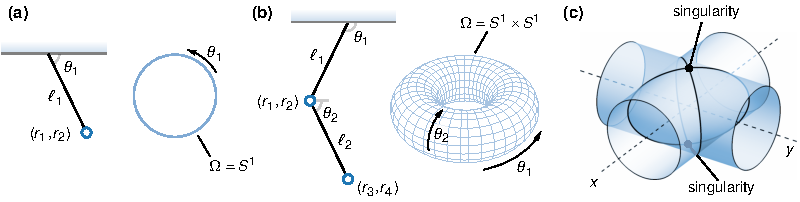
\includegraphics{intro/confspaces.pdf}
  \end{center}
  \caption{
  (a) A simple pendulum and its configuration space $\Sigma = S^{1}$.
  (b) A double pendulum and its configuration space $\Sigma = S^{1} \times S^{1}$.
  (c) Configuration space of a particle constrained to move on two mutually perpendicular cylinders of equal radii is the cylinders' intersection curve, which is not a smooth manifold.
  }
  \label{fig:confspaces}
  % TODO: more descriptive label.
\end{figure}

\subsection{Frameworks}

Soft, few-body systems, composed of a small number of particles or units, interacting via short-ranged forces are commonplace in soft-matter physics.
A paradigmatic example of such a system is a colloidal cluster, which is composed of a small number of colloidal particles with sizes typically ranging from 1~nm to 0.1~$\mu$m.
% TODO: figure of a colloidal cluster and cite papers in the following sentence; plagiarism issues as well.
Colloidal clusters, have been extensively studied both experimentally and theoretically, and provide fundamental insights into a host of phenomena including the formation of nucleation barriers, crystallization, glass transition, etc.
Although the particles in a colloidal cluster are held together by subtle effects of electrostatic and van der Waal forces, such details are often irrelevant if our goal is to describe the more macroscopic properties of the cluster.
To a good approximation, the interactions between the different particles are effectively described using central-force bonds connecting their centers.
Configurations of the resulting ``bond skeleton'', with each bond at its respective rest length, describe the different ground states of the cluster.
Such colloidal skeletons are an example of a mechanical framework, which is an assembly of rigid bars connecting freely-rotating joints.
Frameworks are indeed holonomically-constrained systems, not too different from the examples we have seen so far.
In case of the colloidal cluster, the configuration space of the associated framework is equivalent to the ground-state manifold of the cluster.
%
\begin{figure}
  \begin{center}
    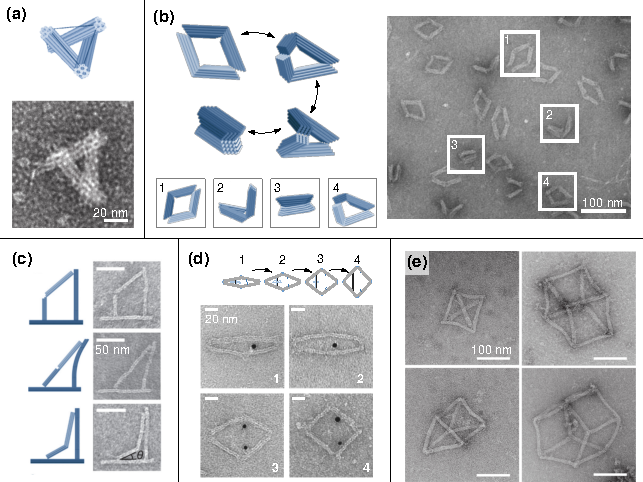
\includegraphics{intro/dna.pdf}
  \end{center}
  \caption{DNA origami has been widely used to self assemble a variety of objects at the nanoscale.
Depicted in the figure are (a) tensegrity structures \cite{liedl2010}; (b), (c) linkage-based mechanisms \cite{marras2015,zhou2015}; (d) a rhombus-shaped nanoactuator~\cite{ke2016}; and (e) self-assembled polyhedra~\cite{iinuma2014}.}
  \label{fig:dna_origami}
\end{figure}



Apart from colloidal clusters, frameworks have been extensively to understand a variety of mechanical structures found in viruses~\cite{hespenheide2004},
crystals~\cite{power2014} and minerals~\cite{kapko2011},
proteins allostery~\cite{gaspar2012}, and of course,
robots and machines~\cite{farber2008,donelan2007}.
In recent years, nanoscale frameworks made out of multihelix DNA bundles (often dubbed ``DNA origami'') have received extensive interest, with applications ranging from drug delivery~\cite{zhao2019} to self assembly~\cite{liedl2010}.
As far as more generic descriptions of thermally-driven frameworks are concerned, there has been long-standing interest in the effect of thermal fluctuations on the mechanical properties of ordered and disordered lattices~\cite{zhang2016,woodhouse2018,yan2018}, and the folding of polymerized membranes~\cite{di-francesco2000,nelson2004} and polyhedral nets~\cite{shenoy2012,dodd2018,melo2020}.
There is, therefore, an arising need to understand how thermal excitations affect the physical properties of these frameworks, but only some attempts have been made so far~\cite{kallus2017,rocklin2018}.

In practice, there is no such thing as a framework with perfect constraints, and it is always possible to violate them by paying some sort of an energy cost.
Multihelix bundles used in DNA origami, for instance, have measured stiffness in the range of 0.1--1~pN$/$nm~\cite{jung2020}.
For realistic frameworks, the configuration space $\Sigma$ would then form the ground-state manifold (assuming that energy costs arise solely due to the constraints being violated).

\subsection{Free energy landscapes}

The effect of thermal fluctuations on a physical system is often represented by its free-energy landscape in terms of a set of collective variables that provide a coarse-grained description of its slowest dynamics.
In theory~\cite{go1976,echenique2011}, one can obtain the free energy of a framework by integrating out the fast modes that are transverse to its shape space, i.e., the subset of its configuration space once rigid-body motions are removed.
Doing this, however, becomes nontrivial when the framework has shape-space singularities~\cite{zlatanov2002,liu2003,donelan2007}.
For concreteness, consider the shape space of the planar four-bar linkage with freely rotating joints~\cite{grashof1883,hartenberg1964,shimamoto2005} (Fig.~\ref{fig:4bar_cs}).
Though this linkage has one degree of freedom up to Euclidean motions, it has two modes of deformation, one where the angle $\theta_1 = \theta_2$ and another where $\theta_1 \ne \theta_2$, meeting at two isolated singular points $(\theta_1,\theta_2) = (0,0)$ and $(\pi,\pi)$.
One generically expects the framework to be soft at these singularities, and indeed, as we see from the blue dashed curves in Fig.~\ref{fig:4bar_collage}(b), the free energy diverges in a harmonic approximation of the elastic energy~\cite{rocklin2018}.
These divergences must be cut off by higher-order nonlinear effects, yet how this happens and to what extent remains to be understood.

In Chapters 2 and 3, we develop a formalism to understand the thermal equilibration of common bar-joint frameworks that have isolated shape-space singularities.
We show that the divergent contributions to the free energy arising in the harmonic approximation to the energy are suppressed by anharmonic, quartic-order corrections.
These findings show the existence of energetic free-energy barriers between configurations near the singularities and configurations farther from the singularities.
Our results are consistent with a closely-related work~\cite{kallus2017,holmes-cerfon2017} on singular colloidal clusters, but allow for isolated singularities of the shape space.
We demonstrate our results using both the four-bar linkage as well as a flat, triangulated origami~\cite{chen2018}.
In addition to these two systems with one-dimensional configuration spaces, we also demonstrate the versatility of our methods using the five-bar linkage, which is a framework with a two-dimensional configuration space.
The analyses presented in these chapters have direct consequences in the design and employment of nanoscale frameworks in applications ranging from self-assembly~\cite{liedl2010} to drug delivery~\cite{zhao2019}, where relative thermodynamic stability of different configurations is of paramount importance.

\begin{figure}
  \begin{center}
    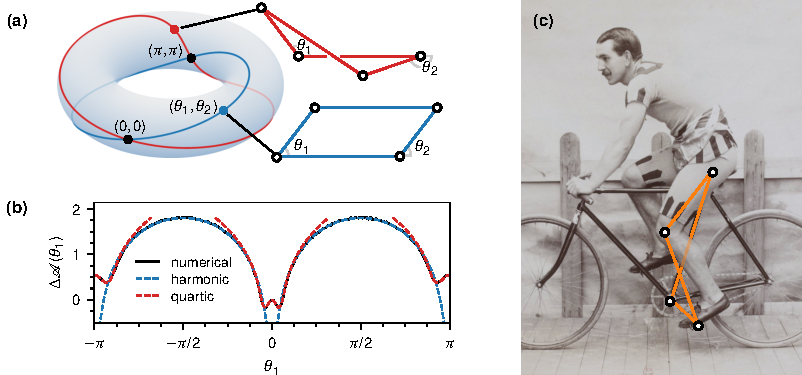
\includegraphics{intro/4bar_collage.pdf}
  \end{center}
\caption{(a) Configuration space of a four-bar linkage visualized as two intersecting curves on a torus. (b) its free energy $\mathscr{A}(\theta_{1})$ as a function of the angle $\theta_{1}$. (c) Four-bar linkage in the real world; photograph by J.~Beau, \emph{Photographie Sportive} (1898).}
  \label{fig:4bar_collage}
\end{figure}

\section{Thin structures, elastic waves, and bound states}

In the second part of this dissertation, we consider the localization of elastic waves in thin elastic structures with spatially varying curvature profiles, using a curved rod and a singly-curved shell as concrete examples.
Previous work on related problems have largely focused on the localization of flexural waves on such structures.
Here, using the semiclassical/WKB approximation, we show that in addition to flexural waves, extensional and shear waves also form localized, bound states around points where the absolute curvature of the structure has a minimum.
These findings open up novel ways to fine-tune the acoustic and vibrational properties of thin elastic structures, and raise the possibility of introducing new phenomena not easily captured by effective models of flexural waves alone.

\subsection{Can one hear the shape of a shell?}

Take an ordinary hand saw used for cutting wood.
Clamp down the handle end of the saw using your feet and bend its tip using your dominant hand into the shape of an $\mathsf{S}$ (see Fig.~\ref{fig:saw} for example).
The saw is now a ``singing'' saw: on bowing or striking it with a mallet, it produces a sharp, sustained sound.
But how does the saw sing and why does it have to be shaped like an \textsf{S}?
The first rigorous answer to this question was provided by \citet{scott1992} who modeled the saw as a thin elastic shell with a varying curvature profile and showed that vibrations get trapped around the saw's inflection point.
Incidentally, saw enthusiasts call the inflection point, where the local curvature vanishes, as the musical ``sweet spot''.
In a very recent work, \citet{shankar2022} argued that the vibrations around the inflection point of a saw are topologically protected.
As trapped waves remain confined to the immediate vicinity of the inflection point, it reduces the energy leakage through the two ends of the saw, resulting in a sustained note.

In this dissertation, we explore other features of curvature-induced localization of elastic waves on thin elastic structures such as rods and shells.
Central to understanding the localization of waves and the formation of bound states in elastodynamic systems, such as the musical saw, is an eigenvalue problem of the form
%
\begin{equation}
  \widehat{\mathsf{D}}\psi = \omega^{2}\psi
  \label{intro:eq:waveeq}
\end{equation}
%
where $\widehat{\mathsf{D}}$ is a differential operator, $\psi$ is the wave field, and $\omega$ is the frequency of vibration.
In the elastodynamic problems involving thin structures, the wave field $\psi$ is almost always composed of displacements---broken up into tangential and normal components---from the neutral, undeformed configuration of the structure.
The operator $\hat{\mathsf{D}}$, the exact nature of which is model dependent, would generally be a matrix of spatial derivatives that act on $\psi$.
An uncurved elastic structure can support three basis wave types: extensional and shear waves, which propagate by stretching the structure and involving only the tangential components [$u$ and $v$ in Fig.~XXX]; and flexural waves that propagate by bending the structure and involving only the normal component [$\zeta$ in Fig.~XXX].
However, if the structure is curved, the normal and tangential components remain coupled, and we can only speak of waves that are predominantly flexural or extensional or shear like. 
%
\begin{figure}
  \begin{center}
    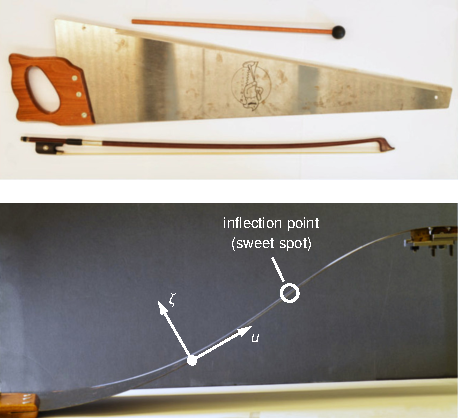
\includegraphics{intro/saw.pdf}
  \end{center}
  \caption{%
    An ordinary hand saw, when bent into the shape of the letter $\mathsf{S}$ can be played like a musical instrument using a violin's bow or a mallet.
    A sustained note is produced on bowing or hitting the saw at its inflection point, which is called a sweet spot by musicians.
    Photographs sourced from Ref.~\cite{shankar2022}.
  }
  \label{fig:saw}
\end{figure}

\subsection{Semiclassical approximation}

Usually, we would look for plane-wave solutions to Eq.~\eqref{intro:eq:waveeq} of the form $\psi \sim e^{\pm i kx}$. 
This, however, is only applicable if the coefficients of the derivatives in $\widehat{\mathsf{D}}$ are constants, which is not the case for a thin structure with a varying curvature profile.\footnote{To be clear, the exact form of the operator $\widehat{\mathsf{D}}$ depends on the shell or rod model we choose to work with, and even when the curvature is a constant, a plain-wave solution may not be applicable.}
The semiclassical approximation or the Wentzel--Krames--Brillouin (WKB) approximation is a widely used method to obtain approximate solutions to differential equations where these coefficients are slowly varying.
In asymptotic analysis, it is usually introduced as an approximate method to find solutions to differential equations whose highest derivative is multiplied by a small parameter~\cite{bender1978}.
A paradigmatic example from physics is the time-independent Schr\"{o}dinger equation for a particle of mass $m$ in a potential $V(x)$
%
\begin{equation}
  \left[-\frac{\hbar^{2}}{2m}\partial_{x}^{2} + V(x)\right]\psi(x) = E\psi(x),
\end{equation}
%
where the WKB method is frequently employed to find asymptotic solutions in the limit the (reduced) Planck's constant $\hbar \to 0$.
At first glance, such a limit makes \emph{no} physical sense as $\hbar$ is a fundamental constant, whose value is fixed by the units we choose to work in.
Rather, in considering the limit $\hbar \to 0$, we are considering the limit where the value of $\hbar$ is much smaller compared to the angular momentum scale, which is often the case with macroscopic systems described by classical physics.%
\footnote{%
  This can be more clearly seen by nondimensionalizing the time-independent Schr\"{o}dinger equation by introducing an energy scale $U$ and a length scale $L$, after which it can be written as
$-\epsilon^{2}\partial_{{x}}^{2}\psi(x) + {V}(x)\psi(x) = {E}\psi(x)$,
where all quantities as well as the parameter $\epsilon = \hbar/\sqrt{2mL^{2}U}$ are now dimensionless.
As $\sqrt{2mL^{2}U}$ has the dimension of the angular momentum, taking the limit $\epsilon \to 0$ is equivalent to saying that typical values of angular momentum is much larger than $\hbar$.}
It is in this context that the WKB method gets the alternative moniker of semiclassical approximation.%
%\footnote{Also known as the quasiclassical method.  In harmonic analysis, the semiclassial approximation is also called semiclassical analysis.  Some others choose to call it the eikonal method and some others call it ray approximation or ray tracing.}

Modern reformulations of the semiclassical method, based on the Weyl symbol calculus, provide unparalleled insights into the connection between classical and quantum mechanics.
Weyl calculus provides an elegant way to construct one-to-one maps between differential operators (i.e., powers of $\partial_{x}$) defined on Hilbert spaces and ordinary functions defined on a position--momentum phase space.
The basic premise is that, under the Weyl transform, the momentum operator $\hat{k} = -i\partial_{x}$ gets mapped to the momentum $k$.
(For simplicity, we have suppressed factors of $\hbar$.)
Thus, after expressing the derivatives of a given differential operator in terms of $\hat{k}$ and its powers, the operator can be mapped to an ordinary function---called its Weyl symbol---defined on an $x$-$k$ phase space, i.e.,
%
% TODO: use tikz instead of harpoons: https:/tex.stackexchange.com/questions/312491/bumpy-uneven-arrows-in-mathtools-mhchem-etc
\begin{equation}
  \widehat{D}\left(x, \partial_{x}\right) = \widehat{D}\left(x, i\hat{k}\right) \quad\text{\small(Hilbert space)} \quad\xrightleftharpoons[\text{Wigner map}]{\text{Weyl transform}}\quad D\left(x, k\right) \quad\text{\small(phase space)}.
\end{equation}
%
The Schr\"{o}dinger operator $\widehat{H} = -\partial_{x}^{2}/2m + V(x)$, for instance, gets mapped to the classical Hamiltonian of a point particle $H(x, k) = k^{2}/2m + V(x)$, as one would expect.
Once the operator is in symbol form, it can be expanded and approximated just like any other ordinary function, which provides a direct path towards obtaining asymptotic solutions to wave equations.

For matrix operators that act on multicomponent wave fields, such as the one in Eq.~\eqref{intro:eq:waveeq}, the corresponding Weyl symbol $\mathsf{D}$ is called the dispersion matrix---an ordinary matrix, whose entries are functions defined on an $x$-$k$ phase space.
The eigenvalues $\lambda(x, k)$ of the dispersion matrix serve as ray Hamiltonians of the different wave types represented by Eq.~\eqref{intro:eq:waveeq}.
This leads us to the phase space representation of waves as rays that satisfy the Hamilton's equations
%
\begin{equation}
\dot{x} = \partial_{k}\lambda(x,k)
\quad\text{and}\quad
\dot{k} = -\partial_{x}\lambda(x, k).
\end{equation}
%
The advantage provided by the semiclassical approximation cannot be overstated: we have effectively reduced the wave equation to a Hamiltonian system describing point particles, a system that is much more easier to analyze.

\subsection{Bound states in thin elastic structures}

The semiclassical approximation also provides a simple way to extract the bound state frequencies by ``quantizing'' the ray trajectories in the phase space.
As we move around a bound orbit, single valuedness of the wave field requires the overall phase to be a half-integral multiple of $2\pi$.
Additional subtleties arise when the wave field has more than one component, which leads to a corrected Bohr--Sommerfeld-type quantization condition of the form
%
\begin{equation}
  \epsilon^{-1}\oint \dd{x}\,k(x) = 2\left(n + \frac{1}{2}\right)\pi - \left(\gamma_{\text{G}} + \gamma_{\text{NG}}\right).
\end{equation}
%
Here $\gamma_{\text{G}}$ and $\gamma_{\text{NG}}$ are extra phases that arise because of the multicomponent nature of the problem.
The phase $\gamma_{\text{G}}$ is a geometric phase~\cite{pancharatnam1956,berry1984}, which was recently shown to be responsible for the toplogical protection of equatorial oceanic waves on the Earth's surface~\cite{venaille2023}.

\section{Organizational summary and other comments}

In the interest of making this dissertation more readable and as as self contained as possible, I have broken up and expanded the two papers I wrote.
This dissertation is organized as follows:
In Chapter 2 we review basic facts about frameworks, their configuration spaces, and derive asymptotic expressions for their elastic energies.
Chapter 3 deals with the effect that thermal fluctuations have on these frameworks, and presents a detailed calculation of the free-energy profiles for three example frameworks.
Chapters 4 and 5 are concerned with the second problem discussed in this dissertation.
In Chapter 4, we review the semiclassical theory of wave phenomena, with special attention paid to multicomponent wave equations.
Chapter 5 is concerned with the application of semiclassical approximation to understand the formation of bound states in thin elastic structures.
Finally, in Appendix~\ref{app:math}, we collect some helpful mathematical results that are used throughout the dissertation.
